The Consistent Boundary Flux technique was devised to 
alleviate the problem of the accuracy of primary variables 
derivatives (mainly velocity and temperature) on boundaries, 
where basis function (nodal) derivatives do not exist.
These derivatives are important since they are needed to compute
the heat flux (and therefore the NUsselt number) or 
dynamic topography and geoid. 


The idea was first introduced in \cite{mizu86} and later used 
in geodynamics \cite{zhgh93}. It was finally implemented 
in the CitcomS code \cite{zhmt08} and more recently
in the ASPECT code (dynamic topography postprocessor).
Note that the CBF should be seen as a post-processor step 
as it does not alter the primary variables values.

The CBF method is implemented and used in \ref{f_XX}.

%---------------------------------------------------------------
\subsubsection{applied to the Stokes equation}
We start from the strong form:
\[
{\bm \nabla}\cdot{\bm \sigma} = {\bm b}
\]
and then write the weak form:
\[
\int_\Omega N {\bm \nabla}\cdot{\bm \sigma} dV = \int_\Omega N {\bm b} dV
\]
where $N$ is any test function. We then use the two equations:
\[
\bm \nabla \cdot ( N  \bm \sigma ) = N \bm \nabla \cdot \bm \sigma + \bm \nabla N \cdot  \bm \sigma  
\quad\quad \text{(chain rule)}
\]
\[
\int_\Omega (\bm \nabla \cdot \bm f )\; dV = \int_\Gamma \bm f\cdot \bm n \; dS
\quad\quad \text{(divergence theorem)}
\]
Integrating the first equation over $\Omega$ and using the second, we can write:
\[
\int_\Gamma N {\bm \sigma}\cdot {\bm n} \; dS 
-  \int_\Omega {\nabla N} \cdot{\bm \sigma} \; dV 
= \int_\Omega N {\bm b} dV
\]
On $\Gamma$, the traction vector is given by ${\bm t}={\bm \sigma}\cdot {\bm n}$: 
\[
\int_\Gamma N {\bm t} dS =  \int_\Omega {\nabla N} \cdot{\bm \sigma} dV + \int_\Omega N {\bm b} dV
\]
Considering the traction vector as an unknown living on the nodes on the boundary, 
we can expand (for $Q_1$ elements)
\[
t_x = \sum_{i=1}^2 t_{x|i} N_i 
\quad\quad
t_y = \sum_{i=1}^2 t_{y|i} N_i 
\]
on the boundary so that the left hand term yields a mass matrix $M'$.
Finally, using our previous experience of discretising the weak form, we can write:
\[
M' \cdot {\cal T} = -\K {\cal V} - \G {\cal P} + f
\]
where ${\cal T}$ is the vector of assembled tractions which we want to compute 
and ${\cal V}$ and ${\cal T}$ are the solutions of the Stokes problem. 
Note that the assembly
only takes place on the elements along the boundary.

Note that the assembled mass matrix is tri-diagonal can be easily solved with 
a Conjugate Gradient method. With a trapezoidal integration rule 
(i.e. Gauss-Lobatto) the matrix can even be diagonalised and the resulting 
matrix is simply diagonal, which results in a very cheap solve \cite{zhgh93}.

%---------------------------------------------------------------
\subsubsection{applied to the heat equation}
We start from the strong form of the heat transfer equation (without the source terms for simplicity):
\[
\rho c_p
\left(\frac{\partial T}{\partial t} + {\bm v}\cdot {\bm \nabla}T\right)
=
{\bm \nabla} \cdot k{\bm \nabla T}
\]
The weak form then writes:
%\[
%\int_\Omega N
%\rho c_p
%\left(\frac{\partial T}{\partial t} + {\bm v}\cdot {\bm \nabla}T\right) dV
%=
%\int_\Omega N
%{\bm \nabla} \cdot k{\bm \nabla T} dV
%\]
\[
\int_\Omega N
\rho c_p
\frac{\partial T}{\partial t} dV 
+
\rho c_p
\int_\Omega N
 {\bm v}\cdot {\bm \nabla}T  dV
=
\int_\Omega N
{\bm \nabla} \cdot k{\bm \nabla T} dV
\]
Using once again integration by parts and divergence theorem:
\[
\int_\Omega N
\rho c_p
\frac{\partial T}{\partial t} dV 
+
\rho c_p
\int_\Omega N
 {\bm v}\cdot {\bm \nabla}T  dV
=
\int_\Gamma N k {\bm \nabla T} \cdot {\bm n} d\Gamma
-
\int_\Omega  {\bm \nabla} N \cdot k{\bm \nabla T} dV
\]
On the boundary we are interested in the heat flux ${\bm q}=-k {\bm \nabla T}$
\[
\int_\Omega N
\rho c_p
\frac{\partial T}{\partial t} dV 
+
\rho c_p
\int_\Omega N
 {\bm v}\cdot {\bm \nabla}T  dV
=
-\int_\Gamma N {\bm q} \cdot {\bm n} d\Gamma
- \int_\Omega  {\bm \nabla} N \cdot k{\bm \nabla T} dV
\]
or,
\[
\int_\Gamma N {\bm q} \cdot {\bm n} d\Gamma
=
-\int_\Omega N
\rho c_p
\frac{\partial T}{\partial t} dV 
-\rho c_p
\int_\Omega N
 {\bm v}\cdot {\bm \nabla}T  dV
- \int_\Omega  {\bm \nabla} N \cdot k{\bm \nabla T} dV
\]
Considering the normal heat flux $q_n = {\bm q} \cdot {\bm n}$ as an unknown 
living on the nodes on the boundary, 
\[
q_n = \sum_{i=1}^2 q_{n|i} N_i
\]
so that the left hand term becomes a mass matrix for the shape functions living on 
the boundary.
We have already covered the right hand side terms when building the FE system 
to solve the heat transport equation, so that in the end 
\[
M' \cdot {\cal Q}_n =
- M \cdot \frac{\partial \bm T}{\partial t} -K_a \cdot {\bm T} - K_d \cdot {\bm T} 
\]
where ${\cal Q}_n$ is the assembled vector of normal heat flux components.
Note that in all terms the assembly only takes place over the elements along the boundary.







\newpage
What follows only applies to the reference element.

\begin{verbatim}
    N
 3-----2
 |     |
W|     |E
 |     |
 0-----1
    S
\end{verbatim}

We start from 
\begin{eqnarray}
\int_{\Gamma} N_i {\bm t} dS 
&=& 
 \int_{\Gamma_{0-1}} N_i {\bm t} dS  
+\int_{\Gamma_{1-2}} N_i {\bm t} dS  
+\int_{\Gamma_{2-3}} N_i {\bm t} dS  
+\int_{\Gamma_{3-0}} N_i {\bm t} dS
\end{eqnarray}
for $i=0,3$. Let us start with $N_0$, then 

\begin{eqnarray}
\int_{\Gamma} N_0 {\bm t} dS 
&=& 
 \int_{\Gamma_{0-1}} N_0 {\bm t} dS  
+\int_{\Gamma_{1-2}} N_0 {\bm t} dS  
+\int_{\Gamma_{2-3}} N_0 {\bm t} dS  
+\int_{\Gamma_{3-0}} N_0 {\bm t} dS \nn\\
&=& \int_{\Gamma_{0-1}} N_0 (N_0^\Gamma {\bm t}_0 + N_1^\Gamma {\bm t}_1) dS \nn\\ 
&+& \int_{\Gamma_{1-2}} N_0 (N_1^\Gamma {\bm t}_1 + N_2^\Gamma {\bm t}_2) dS \nn\\
&+& \int_{\Gamma_{2-3}} N_0 (N_2^\Gamma {\bm t}_2 + N_3^\Gamma {\bm t}_3) dS \nn\\
&+& \int_{\Gamma_{3-0}} N_0 (N_3^\Gamma {\bm t}_3 + N_0^\Gamma {\bm t}_0) dS \nn\\ 
&=& \left( \int_{\Gamma_{0-1}} N_0 N_0^\Gamma dS \right) {\bm t}_0 + \left( \int_{\Gamma_{0-1}} N_0 N_1^\Gamma dS\right) {\bm t}_1 \nn\\ 
&+& \left( \int_{\Gamma_{1-2}} N_0 N_1^\Gamma dS \right) {\bm t}_1 + \left( \int_{\Gamma_{1-2}} N_0 N_2^\Gamma dS\right) {\bm t}_2 \nn\\
&+& \left( \int_{\Gamma_{2-3}} N_0 N_2^\Gamma dS \right) {\bm t}_2 + \left( \int_{\Gamma_{2-3}} N_0 N_3^\Gamma dS\right) {\bm t}_3 \nn\\
&+& \left( \int_{\Gamma_{3-0}} N_0 N_3^\Gamma dS \right) {\bm t}_3 + \left( \int_{\Gamma_{3-0}} N_0 N_0^\Gamma dS\right) {\bm t}_0 \nn  
\end{eqnarray}

In what follows we will make use of 
\[
\int_{-1}^{+1} \frac{1}{4} (1-x)(1-x) dx = 2/3 
\]
\[
\int_{-1}^{+1} \frac{1}{4} (1+x)(1+x) dx = 2/3 
\]
\[
\int_{-1}^{+1} \frac{1}{4} (1+x)(1-x) dx = 1/3 
\]



\newpage 
\begin{eqnarray}
\int_{\Gamma_{0-1}} N_0(r,s=-1) N_0^\Gamma(r) dS  &=&  \int_{-1}^{+1}\frac{1}{2}(1-r) \cdot  \frac{1}{2}(1-r) dr= 2/3 \nn\\
\int_{\Gamma_{0-1}} N_0(r,s=-1) N_1^\Gamma(r) dS  &=&  \int_{-1}^{+1}\frac{1}{2}(1-r) \cdot  \frac{1}{2}(1+r) dr= 1/3 \nn\\
\int_{\Gamma_{1-2}} N_0(r=+1,s) N_1^\Gamma(s) dS  &=&  \int_{-1}^{+1}\frac{1}{4}(0)(1-s) \cdot  \frac{1}{2}(1-s) ds=0 \nn\\
\int_{\Gamma_{1-2}} N_0(r=+1,s) N_2^\Gamma(s) dS  &=&  \int_{-1}^{+1}\frac{1}{4}(0)(1-s) \cdot  \frac{1}{2}(1+s) ds=0 \nn\\
\int_{\Gamma_{2-3}} N_0(r,s=+1) N_2^\Gamma(r) dS  &=&  -\int_{-1}^{+1}\frac{1}{4}(1-r)(0) \cdot  \frac{1}{2}(1+r) dr=0 \nn\\
\int_{\Gamma_{2-3}} N_0(r,s=+1) N_3^\Gamma(r) dS  &=&  -\int_{-1}^{+1}\frac{1}{4}(1-r)(0) \cdot  \frac{1}{2}(1-r) dr=0 \nn\\
\int_{\Gamma_{3-0}} N_0(r=-1,s) N_3^\Gamma(s) dS  &=&  -\int_{-1}^{+1}\frac{1}{2}(1-s) \cdot  \frac{1}{2}(1+s) ds= -1/3 \nn\\
\int_{\Gamma_{3-0}} N_0(r=-1,s) N_0^\Gamma(s) dS  &=&  -\int_{-1}^{+1}\frac{1}{2}(1-s) \cdot  \frac{1}{2}(1-s) ds= -2/3 \nn
\end{eqnarray}

\begin{eqnarray}
\int_{\Gamma_{0-1}} N_1(r,s=-1) N_0^\Gamma(r) dS  &=&  \int_{-1}^{+1} \frac{1}{2}(1+r)     \cdot  \frac{1}{2}(1-r) dr= 1/3\nn\\
\int_{\Gamma_{0-1}} N_1(r,s=-1) N_1^\Gamma(r) dS  &=&  \int_{-1}^{+1} \frac{1}{2}(1+r)     \cdot  \frac{1}{2}(1+r) dr= 2/3\nn\\
\int_{\Gamma_{1-2}} N_1(r=+1,s) N_1^\Gamma(s) dS  &=&  \int_{-1}^{+1} \frac{1}{2}(1-s)     \cdot  \frac{1}{2}(1-s) ds= 2/3\nn\\
\int_{\Gamma_{1-2}} N_1(r=+1,s) N_2^\Gamma(s) dS  &=&  \int_{-1}^{+1} \frac{1}{2}(1-s)     \cdot  \frac{1}{2}(1+s) ds= 1/3\nn\\
\int_{\Gamma_{2-3}} N_1(r,s=+1) N_2^\Gamma(r) dS  &=&  -\int_{-1}^{+1}\frac{1}{4}(1+r)(0)  \cdot  \frac{1}{2}(1+r) dr= 0\nn\\
\int_{\Gamma_{2-3}} N_1(r,s=+1) N_3^\Gamma(r) dS  &=&  -\int_{-1}^{+1}\frac{1}{4}(1+r)(0)  \cdot  \frac{1}{2}(1-r) dr= 0\nn\\
\int_{\Gamma_{3-0}} N_1(r=-1,s) N_3^\Gamma(s) dS  &=&  -\int_{-1}^{+1}\frac{1}{4}(0)(1-s)  \cdot  \frac{1}{2}(1+s) ds= 0\nn\\
\int_{\Gamma_{3-0}} N_1(r=-1,s) N_0^\Gamma(s) dS  &=&  -\int_{-1}^{+1}\frac{1}{4}(0)(1-s)  \cdot  \frac{1}{2}(1-s) ds= 0\nn
\end{eqnarray}

\begin{eqnarray}
\int_{\Gamma_{0-1}} N_2(r,s=-1) N_0^\Gamma(r) dS  &=&  \int_{-1}^{+1} \frac{1}{4}(1+r)(0)  \cdot  \frac{1}{2}(1-r) dr= 0\nn\\
\int_{\Gamma_{0-1}} N_2(r,s=-1) N_1^\Gamma(r) dS  &=&  \int_{-1}^{+1} \frac{1}{4}(1+r)(0)  \cdot  \frac{1}{2}(1+r) dr= 0\nn\\
\int_{\Gamma_{1-2}} N_2(r=+1,s) N_1^\Gamma(s) dS  &=&  \int_{-1}^{+1} \frac{1}{2}(1+s)     \cdot  \frac{1}{2}(1-s) ds= 1/3 \nn\\
\int_{\Gamma_{1-2}} N_2(r=+1,s) N_2^\Gamma(s) dS  &=&  \int_{-1}^{+1} \frac{1}{2}(1+s)     \cdot  \frac{1}{2}(1+s) ds= 2/3 \nn\\
\int_{\Gamma_{2-3}} N_2(r,s=+1) N_2^\Gamma(r) dS  &=&  -\int_{-1}^{+1}\frac{1}{2}(1+r)     \cdot  \frac{1}{2}(1+r) dr= -2/3\nn\\
\int_{\Gamma_{2-3}} N_2(r,s=+1) N_3^\Gamma(r) dS  &=&  -\int_{-1}^{+1}\frac{1}{2}(1+r)     \cdot  \frac{1}{2}(1-r) dr= -1/3\nn\\
\int_{\Gamma_{3-0}} N_2(r=-1,s) N_3^\Gamma(s) dS  &=&  -\int_{-1}^{+1}\frac{1}{4}(0)(1+s)  \cdot  \frac{1}{2}(1+s) ds= 0\nn\\
\int_{\Gamma_{3-0}} N_2(r=-1,s) N_0^\Gamma(s) dS  &=&  -\int_{-1}^{+1}\frac{1}{4}(0)(1+s)  \cdot  \frac{1}{2}(1-s) ds= 0\nn
\end{eqnarray}

\begin{eqnarray}
\int_{\Gamma_{0-1}} N_3(r,s=-1) N_0^\Gamma(r) dS  &=&  \int_{-1}^{+1} \frac{1}{4}(1-r)(0) \cdot  \frac{1}{2}(1-r) dr= 0\nn\\
\int_{\Gamma_{0-1}} N_3(r,s=-1) N_1^\Gamma(r) dS  &=&  \int_{-1}^{+1} \frac{1}{4}(1-r)(0) \cdot  \frac{1}{2}(1+r) dr= 0\nn\\
\int_{\Gamma_{1-2}} N_3(r=+1,s) N_1^\Gamma(s) dS  &=&  \int_{-1}^{+1} \frac{1}{4}(0)(1+s) \cdot  \frac{1}{2}(1-s) ds= 0\nn\\
\int_{\Gamma_{1-2}} N_3(r=+1,s) N_2^\Gamma(s) dS  &=&  \int_{-1}^{+1} \frac{1}{4}(0)(1+s) \cdot  \frac{1}{2}(1+s) ds= 0\nn\\
\int_{\Gamma_{2-3}} N_3(r,s=+1) N_2^\Gamma(r) dS  &=&  -\int_{-1}^{+1}\frac{1}{2}(1-r)    \cdot  \frac{1}{2}(1+r) dr= -1/3\nn\\
\int_{\Gamma_{2-3}} N_3(r,s=+1) N_3^\Gamma(r) dS  &=&  -\int_{-1}^{+1}\frac{1}{2}(1-r)    \cdot  \frac{1}{2}(1-r) dr= -2/3\nn\\
\int_{\Gamma_{3-0}} N_3(r=-1,s) N_3^\Gamma(s) dS  &=&  -\int_{-1}^{+1}\frac{1}{2}(1+s)    \cdot  \frac{1}{2}(1+s) ds= -2/3\nn\\
\int_{\Gamma_{3-0}} N_3(r=-1,s) N_0^\Gamma(s) dS  &=&  -\int_{-1}^{+1}\frac{1}{2}(1+s)    \cdot  \frac{1}{2}(1-s) ds= -1/3\nn
\end{eqnarray}







\newpage
so finally
\begin{eqnarray}
\int_{\Gamma} N_0 {\bm t} dS &=& \frac{1}{3} {\bm t}_1 -  \frac{1}{3} {\bm t}_3  \nn\\ 
\int_{\Gamma} N_1 {\bm t} dS &=& \frac{1}{3} {\bm t}_0 + \frac{4}{3} {\bm t}_1 +  \frac{1}{3} {\bm t}_2 \nn\\   
\int_{\Gamma} N_2 {\bm t} dS &=& \frac{1}{3} {\bm t}_1  -\frac{1}{3}  {\bm t}_3\nn\\ 
\int_{\Gamma} N_3 {\bm t} dS &=& -\frac{1}{3} {\bm t}_0 - \frac{1}{3} {\bm t}_2 - \frac{4}{3} {\bm t}_3 \nn
\end{eqnarray}
 
\[
\frac{1}{3}
\left(
\begin{array}{cccccccc}
. &. &1 &. &. &. &-1 & .\\
.& . &. &1 &. &. &. &-1 \\
1 & . & 4 & . & 1 &. & .& .\\
. &1 & . & 4 & . & 1 &. & . \\
. & . & 1 & .& . & . & -1 & .\\
. & . & . & 1 & .& . & . & -1 \\
-1 & . & . & . & -1 & .  & -4 & . \\
. & -1 & . & . & . & -1 & .  & -4  
\end{array}
\right)
\cdot
\left(
\begin{array}{c}
t_{x,0}\\
t_{y,0}\\
t_{x,1}\\
t_{y,1}\\
t_{x,2}\\
t_{y,2}\\
t_{x,3}\\
t_{y,3}
\end{array}
\right)
=
\left(
\begin{array}{c}
\\
\\
\\
rhs\\
\\
\\
\\
\end{array}
\right)
\]
Note that the resulting matrix is symmetric.


\newpage
Let us start with a small example, a 3x2 element FE grid:
\begin{center}
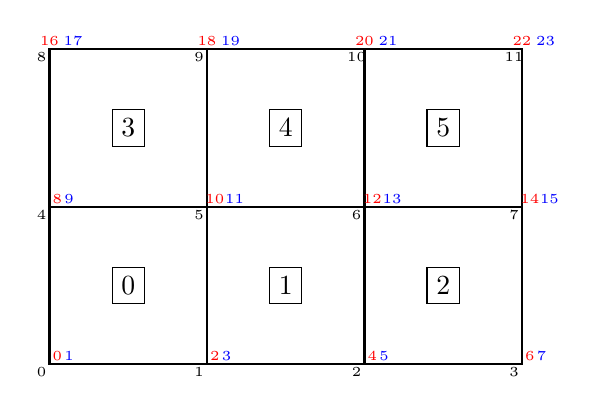
\begin{tikzpicture}
%\draw[step=0.5cm,gray,very thin] (0,0) grid (8,6); %background grid
\draw[thick] (1,1) -- (3,1) -- (3,3) -- (1,3) -- cycle;  
\draw[thick] (3,1) -- (5,1) -- (5,3) -- (3,3) -- cycle; 
\draw[thick] (5,1) -- (7,1) -- (7,3) -- (5,3) -- cycle; 
\draw[thick] (1,3) -- (3,3) -- (3,5) -- (1,5) -- cycle;  
\draw[thick] (3,3) -- (5,3) -- (5,5) -- (3,5) -- cycle; 
\draw[thick] (5,3) -- (7,3) -- (7,5) -- (5,5) -- cycle; 
\node[draw] at (2,2) {0};
\node[draw] at (4,2) {1};
\node[draw] at (6,2) {2};
\node[draw] at (2,4) {3};
\node[draw] at (4,4) {4};
\node[draw] at (6,4) {5};
%pressure dofs
\node at (0.9,0.9) {\tiny 0};
\node at (2.9,0.9) {\tiny 1};
\node at (4.9,0.9) {\tiny 2};
\node at (6.9,0.9) {\tiny 3};
\node at (0.9,2.9) {\tiny 4};
\node at (2.9,2.9) {\tiny 5};
\node at (4.9,2.9) {\tiny 6};
\node at (6.9,2.9) {\tiny 7};
\node at (0.9,4.9) {\tiny 8};
\node at (2.9,4.9) {\tiny 9};
\node at (4.9,4.9) {\tiny 10};
\node at (6.9,4.9) {\tiny 11};
%velocity dofs
\node[red] at (1.1,1.1) {\tiny 0};  \node[blue] at (1.25,1.1) {\tiny 1};
\node[red] at (3.1,1.1) {\tiny 2};  \node[blue] at (3.25,1.1) {\tiny 3};
\node[red] at (5.1,1.1) {\tiny 4};  \node[blue] at (5.25,1.1) {\tiny 5};
\node[red] at (7.1,1.1) {\tiny 6};  \node[blue] at (7.25,1.1) {\tiny 7};
\node[red] at (1.1,3.1) {\tiny 8};  \node[blue] at (1.25,3.1) {\tiny 9};
\node[red] at (3.1,3.1) {\tiny 10}; \node[blue] at (3.35,3.1) {\tiny 11};
\node[red] at (5.1,3.1) {\tiny 12}; \node[blue] at (5.35,3.1) {\tiny 13};
\node[red] at (7.1,3.1) {\tiny 14}; \node[blue] at (7.35,3.1) {\tiny 15};
\node[red] at (1.,5.1) {\tiny 16}; \node[blue] at (1.3,5.1) {\tiny 17};
\node[red] at (3.,5.1) {\tiny 18}; \node[blue] at (3.3,5.1) {\tiny 19};
\node[red] at (5.,5.1) {\tiny 20}; \node[blue] at (5.3,5.1) {\tiny 21};
\node[red] at (7.,5.1) {\tiny 22}; \node[blue] at (7.3,5.1) {\tiny 23};
\end{tikzpicture}\\
{\tiny Red color corresponds to the dofs in the x direction, blue color indicates a dof in the y direction.}
\end{center}

We have nnp=12, nel=6, NfemV=24. Let us assume that free slip boundary conditions are applied. 
The {\tt fix\_bc} array is then:
\begin{center}
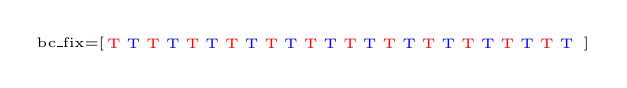
\begin{tikzpicture}
%\draw[step=0.5cm,gray,very thin] (0,0) grid (9,0.7); %background grid
\node  at (0.45,.1) {\tiny bc\_fix=[};

\node[red]  at (1.00,.1) {\tiny T};
\node[blue] at (1.25,.1) {\tiny T};
\node[red]  at (1.50,.1) {\tiny T};
\node[blue] at (1.75,.1) {\tiny T};
\node[red]  at (2.00,.1) {\tiny T};
\node[blue] at (2.25,.1) {\tiny T};
\node[red]  at (2.50,.1) {\tiny T};
\node[blue] at (2.75,.1) {\tiny T};
\node[red]  at (3.00,.1) {\tiny T};
\node[blue] at (3.25,.1) {\tiny T};
\node[red]  at (3.50,.1) {\tiny T};
\node[blue] at (3.75,.1) {\tiny T};
\node[red]  at (4.00,.1) {\tiny T};
\node[blue] at (4.25,.1) {\tiny T};
\node[red]  at (4.50,.1) {\tiny T};
\node[blue] at (4.75,.1) {\tiny T};
\node[red]  at (5.00,.1) {\tiny T};
\node[blue] at (5.25,.1) {\tiny T};
\node[red]  at (5.50,.1) {\tiny T};
\node[blue] at (5.75,.1) {\tiny T};
\node[red]  at (6.00,.1) {\tiny T};
\node[blue] at (6.25,.1) {\tiny T};
\node[red]  at (6.50,.1) {\tiny T};
\node[blue] at (6.75,.1) {\tiny T};

\node  at (7,.1) {\tiny ]};

\end{tikzpicture}\\
\end{center}
Note that since corners belong to two edges, we effectively prescribed 
no-slip boundary conditions on those. 

We wish to compute the tractions on the boundaries, and more precisely for the dofs for which 
a Dirichlecht velocity boundary condition has been prescribed.
The number of (traction) unknowns NfemTr is then the number of {\tt T} in the {\tt bc\_fix} array.
In our specific case, we wave NfemTr= .
This means that we need for each targeted dof to be able to find its identity/number
between 0 and NfemTr-1. We therefore create the array {\tt bc\_nb} which is 
filled as follows: 
 
\begin{center}
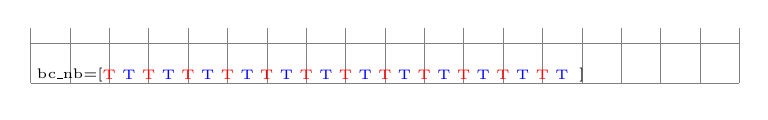
\begin{tikzpicture}
\draw[step=0.5cm,gray,very thin] (0,0) grid (9,0.7); %background grid

\node  at (0.5,.1) {\tiny bc\_nb=[};

\node[red]  at (1.00,.1) {\tiny T};
\node[blue] at (1.25,.1) {\tiny T};
\node[red]  at (1.50,.1) {\tiny T};
\node[blue] at (1.75,.1) {\tiny T};
\node[red]  at (2.00,.1) {\tiny T};
\node[blue] at (2.25,.1) {\tiny T};
\node[red]  at (2.50,.1) {\tiny T};
\node[blue] at (2.75,.1) {\tiny T};
\node[red]  at (3.00,.1) {\tiny T};
\node[blue] at (3.25,.1) {\tiny T};
\node[red]  at (3.50,.1) {\tiny T};
\node[blue] at (3.75,.1) {\tiny T};
\node[red]  at (4.00,.1) {\tiny T};
\node[blue] at (4.25,.1) {\tiny T};
\node[red]  at (4.50,.1) {\tiny T};
\node[blue] at (4.75,.1) {\tiny T};
\node[red]  at (5.00,.1) {\tiny T};
\node[blue] at (5.25,.1) {\tiny T};
\node[red]  at (5.50,.1) {\tiny T};
\node[blue] at (5.75,.1) {\tiny T};
\node[red]  at (6.00,.1) {\tiny T};
\node[blue] at (6.25,.1) {\tiny T};
\node[red]  at (6.50,.1) {\tiny T};
\node[blue] at (6.75,.1) {\tiny T};
\node  at (7,.1) {\tiny ]};
\end{tikzpicture}\\
\end{center}

This translates as follows in the code:
\begin{lstlisting}
NfemTr=np.sum(bc_fix)
bc_nb=np.zeros(NfemV,dtype=np.int32)
counter=0
for i in range(0,NfemV):
    if (bc_fix[i]):
       bc_nb[i]=counter
       counter+=1
\end{lstlisting}







The algorithm is then as follows

\begin{itemize}
\item[A] Prepare two arrays to store the matrix $M_{cbf}$ and its right hand side $rhs_{cbf}$  

\item[B] 
Loop over all elements 

\item[C] 
For each element touching a boundary, compute the residual vector 
$R_{el}=-f_{el} + \K_{el}{\cal V}_{el} + \G_{el} {\cal P}_{el}$

\item[D]
Loop over the four edges of the element using the connectivity array

\item[E]
For each edge loop over the number of degrees of freedom (2 in 2D)

\item[F] 
For each edge assess whether the dofs on both ends are target dofs. 

\item[G]
If so, compute the mass matrix $M_{edge}$ for this edge 

\item[H] extract the 2 values off the element residual vector and assemble these
in $rhs_{cbf}$

\item[I] Assemble $M_{edge}$ into NfemTrxNfemTr matrix using bc\_nb
\end{itemize}


\begin{lstlisting}
M_cbf = np.zeros((NfemTr,NfemTr),np.float64)         # A
rhs_cbf = np.zeros(NfemTr,np.float64)

for iel in range(0,nel):                             # B

    ... compute elemental residual ...               # C

    #boundary 0-1                                    # D
    for i in range(0,ndofV):                         # E
        idof0=2*icon[0,iel]+i
        idof1=2*icon[1,iel]+i
        if (bc_fix[idof0] and bc_fix[idof1]):        # F
           idofTr0=bc_nb[idof0]   
           idofTr1=bc_nb[idof1]
           rhs_cbf[idofTr0]+=res_el[0+i]             # H
           rhs_cbf[idofTr1]+=res_el[2+i]              
           M_cbf[idofTr0,idofTr0]+=M_edge[0,0]       # 
           M_cbf[idofTr0,idofTr1]+=M_edge[0,1]       # I
           M_cbf[idofTr1,idofTr0]+=M_edge[1,0]       # 
           M_cbf[idofTr1,idofTr1]+=M_edge[1,1]       #

    #boundary 1-2                                    #[D]

    ...

    #boundary 2-3                                    #[D]

    ...

    #boundary 3-0                                    #[D]

    ...


\end{lstlisting}



































\newpage
\begin{eqnarray}
\text{Element 0:} \quad\quad
\int_{\Gamma} N_i {\bm t} dS 
&=& \int_{\Gamma_{0-1}} N_i {\bm t} dS  +\int_{\Gamma_{1-5}} N_i {\bm t} dS +\int_{\Gamma_{5-4}} N_i {\bm t} dS  +\int_{\Gamma_{4-0}} N_i {\bm t} dS\\
\text{Element 1:} \quad\quad
\int_{\Gamma} N_i {\bm t} dS 
&=& \int_{\Gamma_{1-2}} N_i {\bm t} dS  +\int_{\Gamma_{2-6}} N_i {\bm t} dS +\int_{\Gamma_{6-5}} N_i {\bm t} dS  +\int_{\Gamma_{5-1}} N_i {\bm t} dS\\
\text{Element 2:} \quad\quad
\int_{\Gamma} N_i {\bm t} dS 
&=& \int_{\Gamma_{2-3}} N_i {\bm t} dS  +\int_{\Gamma_{3-7}} N_i {\bm t} dS +\int_{\Gamma_{7-6}} N_i {\bm t} dS  +\int_{\Gamma_{6-2}} N_i {\bm t} dS\\
\text{Element 3:} \quad\quad
\int_{\Gamma} N_i {\bm t} dS 
&=& \int_{\Gamma_{4-5}} N_i {\bm t} dS  +\int_{\Gamma_{5-9}} N_i {\bm t} dS +\int_{\Gamma_{9-8}} N_i {\bm t} dS  +\int_{\Gamma_{8-4}} N_i {\bm t} dS\\
\text{Element 4:} \quad\quad
\int_{\Gamma} N_i {\bm t} dS 
&=& \int_{\Gamma_{5-6}} N_i {\bm t} dS  +\int_{\Gamma_{6-10}} N_i {\bm t} dS +\int_{\Gamma_{10-9}} N_i {\bm t} dS  +\int_{\Gamma_{9-5}} N_i {\bm t} dS\\
\text{Element 5:} \quad\quad
\int_{\Gamma} N_i {\bm t} dS 
&=& \int_{\Gamma_{6-7}} N_i {\bm t} dS  +\int_{\Gamma_{7-11}} N_i {\bm t} dS +\int_{\Gamma_{11-10}} N_i {\bm t} dS  +\int_{\Gamma_{10-6}} N_i {\bm t} dS
\end{eqnarray}

We see that the integral $\int_{\Gamma_{1-5}} N_i {\bm t} dS$ of element 0 is exactly the opposite\footnote{these are line integrals, one is going from node 1 to 5, the other from 5 to 1} of the the integral $\int_{\Gamma_{5-1}} N_i {\bm t} dS$ of element 1, so that their contributions to the assembled matrix 
would actually cancel out. Likewise, any edge common to two elements will see in the expressions above two integrals of opposite sign, shich ultimately will not
contribute to the assembled matrix. 

Let us then remove the integrals over edges 1-5, 2-6, 4-5, 5-6, 6-7, 5-9 and 6-10 off the equations above:

\begin{eqnarray}
\text{Element 0:} \quad\quad
\int_{\Gamma} N_i {\bm t} dS 
&=& \int_{\Gamma_{0-1}} N_i {\bm t} dS  +\int_{\Gamma_{4-0}} N_i {\bm t} dS\\
&=& \int_{\Gamma_{0-1}} N_i (N_0 {\bm t}_0 + N_1 {\bm t}_1)  dS  +\int_{\Gamma_{4-0}} N_i (N_0 {\bm t}_0 +N_4 {\bm t}_4) dS\\
&=& \int_{\Gamma_{0-1}} N_i N_0 dS \quad {\bm t}_0  +  \int_{\Gamma_{0-1}} N_i N_1 dS \quad  {\bm t}_1  
+\int_{\Gamma_{4-0}} N_i N_0 dS \quad  {\bm t}_0 + \int_{\Gamma_{4-0}} N_i N_4 dS \quad {\bm t}_4 \nonumber\\
\text{Element 1:} \quad\quad
\int_{\Gamma} N_i {\bm t} dS 
&=& \int_{\Gamma_{1-2}} N_i {\bm t} dS  \\ 
&=& \int_{\Gamma_{1-2}} N_i (N_1 {\bm t}_1 + N_2 {\bm t}_2) dS  \\ 
\text{Element 2:} \quad\quad
\int_{\Gamma} N_i {\bm t} dS 
&=& \int_{\Gamma_{2-3}} N_i {\bm t} dS  +\int_{\Gamma_{3-7}} N_i {\bm t} dS \\ 
\text{Element 3:} \quad\quad
\int_{\Gamma} N_i {\bm t} dS 
&=& \int_{\Gamma_{9-8}} N_i {\bm t} dS  +\int_{\Gamma_{8-4}} N_i {\bm t} dS\\
\text{Element 4:} \quad\quad
\int_{\Gamma} N_i {\bm t} dS 
&=& \int_{\Gamma_{10-9}} N_i {\bm t} dS \\ 
&=& \int_{\Gamma_{10-9}} N_i (N_{10}{\bm t}_{10}+N_{9}{\bm t}_9) dS \\ 
\text{Element 5:} \quad\quad
\int_{\Gamma} N_i {\bm t} dS 
&=& \int_{\Gamma_{7-11}} N_i {\bm t} dS +\int_{\Gamma_{11-10}} N_i {\bm t} dS  
\end{eqnarray}
We see that the 


































